%%%%%%%%%%%%%%%%%%%%%%%%%%%%%%%%%%%%%%%%%%%%%%%%%%%%%%%%%%%%%%%%%%%%%%%%%%%%%%%%
% Template for USENIX papers.
%
% History:
%
% - TEMPLATE for Usenix papers, specifically to meet requirements of
%   USENIX '05. originally a template for producing IEEE-format
%   articles using LaTeX. written by Matthew Ward, CS Department,
%   Worcester Polytechnic Institute. adapted by David Beazley for his
%   excellent SWIG paper in Proceedings, Tcl 96. turned into a
%   smartass generic template by De Clarke, with thanks to both the
%   above pioneers. Use at your own risk. Complaints to /dev/null.
%   Make it two column with no page numbering, default is 10 point.
%
% - Munged by Fred Douglis <douglis@research.att.com> 10/97 to
%   separate the .sty file from the LaTeX source template, so that
%   people can more easily include the .sty file into an existing
%   document. Also changed to more closely follow the style guidelines
%   as represented by the Word sample file.
%
% - Note that since 2010, USENIX does not require endnotes. If you
%   want foot of page notes, don't include the endnotes package in the
%   usepackage command, below.
% - This version uses the latex2e styles, not the very ancient 2.09
%   stuff.
%
% - Updated July 2018: Text block size changed from 6.5" to 7"
%
% - Updated Dec 2018 for ATC'19:
%
%   * Revised text to pass HotCRP's auto-formatting check, with
%     hotcrp.settings.submission_form.body_font_size=10pt, and
%     hotcrp.settings.submission_form.line_height=12pt
%
%   * Switched from \endnote-s to \footnote-s to match Usenix's policy.
%
%   * \section* => \begin{abstract} ... \end{abstract}
%
%   * Make template self-contained in terms of bibtex entires, to allow
%     this file to be compiled. (And changing refs style to 'plain'.)
%
%   * Make template self-contained in terms of figures, to
%     allow this file to be compiled. 
%
%   * Added packages for hyperref, embedding fonts, and improving
%     appearance.
%   
%   * Removed outdated text.
%
%%%%%%%%%%%%%%%%%%%%%%%%%%%%%%%%%%%%%%%%%%%%%%%%%%%%%%%%%%%%%%%%%%%%%%%%%%%%%%%%

\documentclass[letterpaper,twocolumn,10pt]{article}
\usepackage{usenix2019_v3}

% to be able to draw some self-contained figs
\usepackage{tikz}
\usepackage{amsmath}

% inlined bib file
\usepackage{filecontents}

%-------------------------------------------------------------------------------
\begin{filecontents}{\jobname.bib}
%-------------------------------------------------------------------------------
@Book{arpachiDusseau18:osbook,
  author =       {Arpaci-Dusseau, Remzi H. and Arpaci-Dusseau Andrea C.},
  title =        {Operating Systems: Three Easy Pieces},
  publisher =    {Arpaci-Dusseau Books, LLC},
  year =         2015,
  edition =      {1.00},
  note =         {\url{http://pages.cs.wisc.edu/~remzi/OSTEP/}}
}
@InProceedings{waldspurger02,
  author =       {Waldspurger, Carl A.},
  title =        {Memory resource management in {VMware ESX} server},
  booktitle =    {USENIX Symposium on Operating System Design and
                  Implementation (OSDI)},
  year =         2002,
  pages =        {181--194},
  note =         {\url{https://www.usenix.org/legacy/event/osdi02/tech/waldspurger/waldspurger.pdf}}}
\end{filecontents}

%-------------------------------------------------------------------------------
\begin{document}
%-------------------------------------------------------------------------------

%don't want date printed
\date{}

% make title bold and 14 pt font (Latex default is non-bold, 16 pt)
\title{\Large \bf CS131 Project Report: Proxy Herd with Asyncio}

%for single author (just remove % characters)
\author{
{\rm Melody Chen}\\
Discussion 1C
% copy the following lines to add more authors
% \and
% {\rm Name}\\
%Name Institution
} % end author

\maketitle

%-------------------------------------------------------------------------------
\begin{abstract}
%-------------------------------------------------------------------------------
In this project, we explored how to implement a Proxy herd in Python using the ayncio asynchronous networking library. We also researched whether asyncio library is suitable framework for implementing an "application server herd", where multiple application servers communicate directly to each other as well as via core database and caches.  We compare our implementation in Python to a Java-based approach and compare the overall approach of asyncio with that of Node.js.
\end{abstract}


%-------------------------------------------------------------------------------
\section{Introduction}
%-------------------------------------------------------------------------------
Wikipedia is based on the Wikimedia server platform that is build using GNU/Linus, Apache, MariaDB, and PHP+Javascript, which works well for Wikipedia but not necessarily for a new Wikimedia-style service designed for news with the following specifications:
(1) updates to articles will happen far more often (2) access will be required via various protocols, not just HTTP (3) clients will tend to be more mobile. \par
With the following specifications, the current implementation of the Wikimedia server is not suitable as new servers will need to be added and the response time will be too slow due to bottleneck for the application server. We consider a different type of architecture called the "application server herd", where we have multiple application servers that can communicate with each other in addition to core database and caches. This architecture allows for interserver communication without and transmission of data without bottleneck in current implementation of Wikimedia server. Instead of just connecting to one single server, clients can connect to any server in the herd and the data will be propagated to the neighboring servers without having to access the database.
\par
In this project, we focus on exploring the implementation of the "application server herd" in Python, and specifically the asyncio synchronous networking library. Asyncio is a single-threaded approach for concurrent programming, which differs from parallel programming. Using the asyncio library we build a prototype server herd that consist of five servers that can communicate directly to each other. Through the prototype, we evaluate whether Python and the asyncio framework is suitable for building the new Wikimedia-style service with the specifications mentioned above.

%-------------------------------------------------------------------------------
\section{Python, Java, and the Asyncio Library}
%-------------------------------------------------------------------------------
In this section, we evaluate Python's type checking, memory management, multi-threading approach and compare them to a Java-based approach. We proceed to talk about functionalities of the Asyncio Library in Python.
\subsection{Type Checking}
Python is a dynamically typed language, which means the Python interpreter does type checking as the code is being run and Python variables are allowed to have different types throughout the program. The major upside of having dynamic typing is that this makes the language a lot simpler and more concise, as all declarations are shorter. This makes code written in Python more readable. Another upside that makes implementing server herd in Python a lot simpler is that variables/objects can be passed between different functions/modules without having to know or declare their types. This means that we can use built-in functions of different libraries, in our case, the Asyncio library, without knowing the exact type of every parameter. \par
In contrast, Java is a static typing language where checks are performed without running the program, typically when the program is compiled. Generally, variables are not allowed to change types overtime. The advantage of static typing is that type errors can be caught early, so during run-time there will be no type errors. Thus, for larger, more complicated application, it may be safer to write code in Java to avoid run-time errors. 
\subsection{Memory Management}
Both Python and Java uses Garbage Collectors, however the two implementations are very different. Python's garbage collection method is relatively simple, it is based on the idea of reference counts. As soon as the reference count of an object reaches 0, the object's memory is automatically freed. The advantage of Python's Garbage Collection is that it is simple and fast to keep track of reference counts of all objects. Nevertheless, it is inefficient against circular references, as reference counts for circularly linked objects will always be non-zero. In our herd server implementation, there is not likely going to be circular references, which makes Python a good choice for implementation in terms of memory management.\par
In contrast, Java's garbage collection periodically runs the mark-and-sweep algorithm to determine which objects are no longer in use. The algorithm traverses all object references beginning from roots of object trees and marks every object it can reach. The rest of the heap memory that cannot be reached will be freed. The benefit of Java's implementation over Python's is that it is effective against circular references. Nevertheless, it is more complicated to implement and run in constrast to Python's simple reference count method.
\subsection{Multithreading}
In Python, the Global Interpreter Lock(GIL) guarantees only one thread who holds the lock can be executed at one time, which means there is no parallel threading in Python. This design may seem limiting at first, but Python does this because of its simple garbage collection method. In Python, as soon as reference count of an object reaches 0, the object's memory is released. With multi-threading, the chances of memory leaks increases with Python's garbage collection model. \par
We can compare this to Java's Memory Model where multi-threading is allowed and there is also garbage collection. With Java's choice of allowing for multi-threading, it increases its risks of race condition and relies on more complicated synchronization methods and locks to avoid race conditions. In contrast, Python programs have no need to spend time to acquire or release locks, which allows it to execute fast single-threading code. GIL also allows Python to use C libraries that are not thread-safe. Even with GIL, Python still supports multi-threading. Instead of running them at the same time, Python switches running threads. \par
For the current purpose of our server herds, a single-threaded program will be able to accomplish the purpose, as each server is not doing heavy duty computation that can benefit from multi-threading each time it receives a request. 
\subsection{Asyncio Library}
In this project, we use the Asyncio library which supports multitasking in Python to implement our server herd. The Asyncio library is a single-threaded approach for concurrent programming. It is a cooperative multitasking library in which tasks can voluntarily yield to let other tasks run and the library can also be used to write TCP clients/servers. Main concepts in the Asyncio library are the two following keywords:
\begin{description}
\item[async] Defines a function that is a coroutine which can suspend its execution and allow another coroutine to run
\item[await] Suspends execution of current coroutine until awaited action is finished
\end{description}
The event loop is the core of every Asyncio application. Tasks are executed in an event loop, and whenever a task suspends its execution and yields, another task from the queue can be executed in the event loop as shown in Figure 1. \par
%---------------------------
\begin{figure}
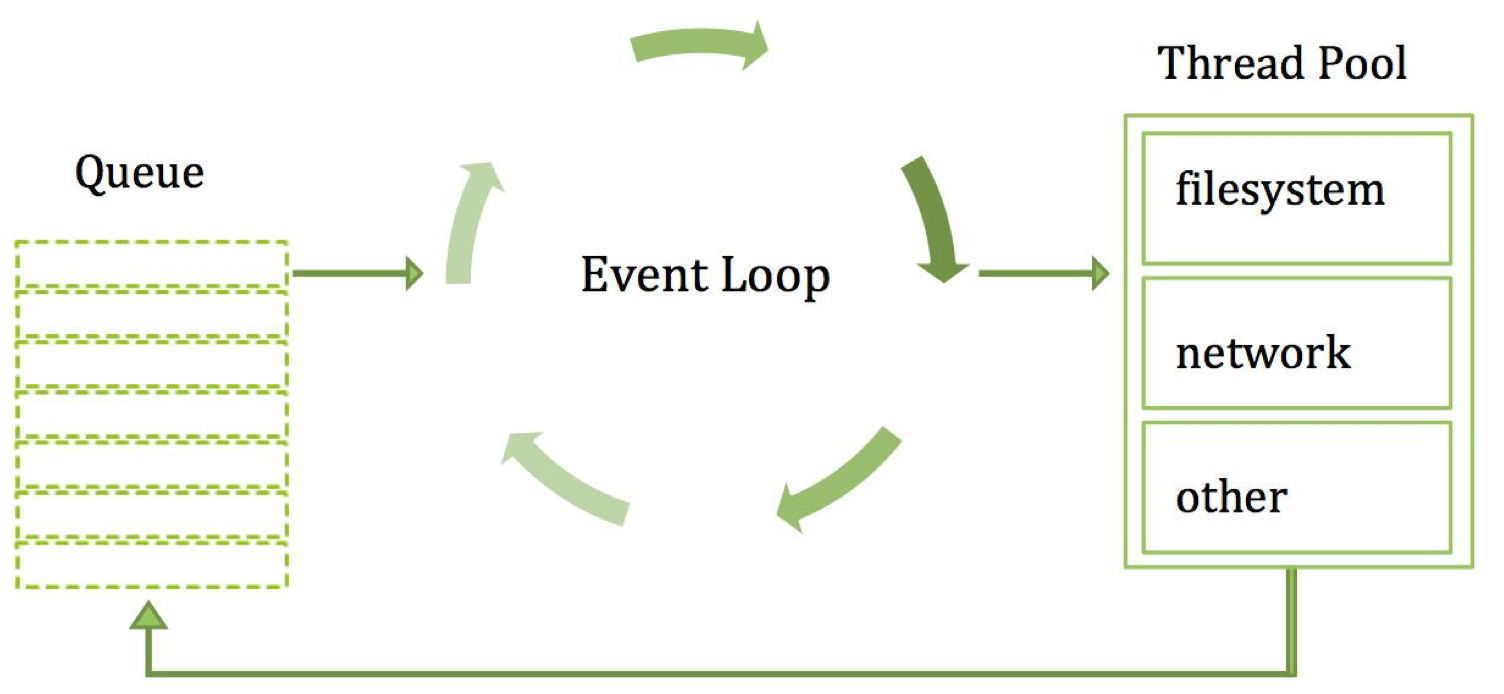
\includegraphics[scale=0.3]{eventloop.png}
\caption{\label{fig:vectors} Diagram of Event Loops in Asyncio(from Discussion 1A Slides)}
\end{figure}
%% %---------------------------
The Asyncio library can also be used to write TCP clients/servers. Servers in Asyncio are set up with an event loop that can process requests that are in the form of coroutines. Every time a request from a client comes in, server receives the request in the form of coroutine. With built-in functions from the Asyncio library, servers that can handle multiple requests are easily implemented.


%-------------------------------------------------------------------------------
\section{Implementation of Server Herd Prototype}
%-------------------------------------------------------------------------------
We're tasked with building a server herd that can synchronize data and communicate with client applications using the Asyncio library. The server herd will act as a simple and parallelizable proxy for the Google Places API. Our server herd has five servers with the names: Jaquez, Hill, Smith, Singleton, and Campbell. Connections between servers are shown in Figure 2. Clients can connect with any of the five servers and send either IAMAT Requests or WHATSAT Requests. All other requests are considered invalid and will be return to the client in the following form:
\begin{center}
    ? <Invalid Message>
\end{center}
Each server is started with built-in \texttt{start\_server} function provided by the Asyncio library that starts a socket server and returns a pair of (reader, writer) objects that server can use to read data from client and send data to client.

\subsection{IAMAT Requests}
IAMAT Requests are sent from clients to update the servers about its current location in coordinates. The requests are of the following form:
\begin{center}
    IAMAT <Client ID> <Coordinates> <Timestamp>
\end{center}
Coordinates are specified using the ISO 6709 notation and timestamp is expressed in POSIX time. Once a server receives an IAMAT Request, it stores the information received and propagates that information to other connected servers through a flooding algorithm. In Python, location and timestamp of client can easily be stored in a dictionary. To prevent flooding algorithm from looping infinitely, every time we received a propagated message, we check whether we have already received the message previously via information stored in local server dictionaries. \par
Once information regarding client is properly flooded to all other server, we respond to the client, signifying that we have received the request, in the following format:
\begin{center}
    AT <Time Difference> <Client ID> <Coordinates> <Timestamp>
\end{center}
%---------------------------
\begin{figure}
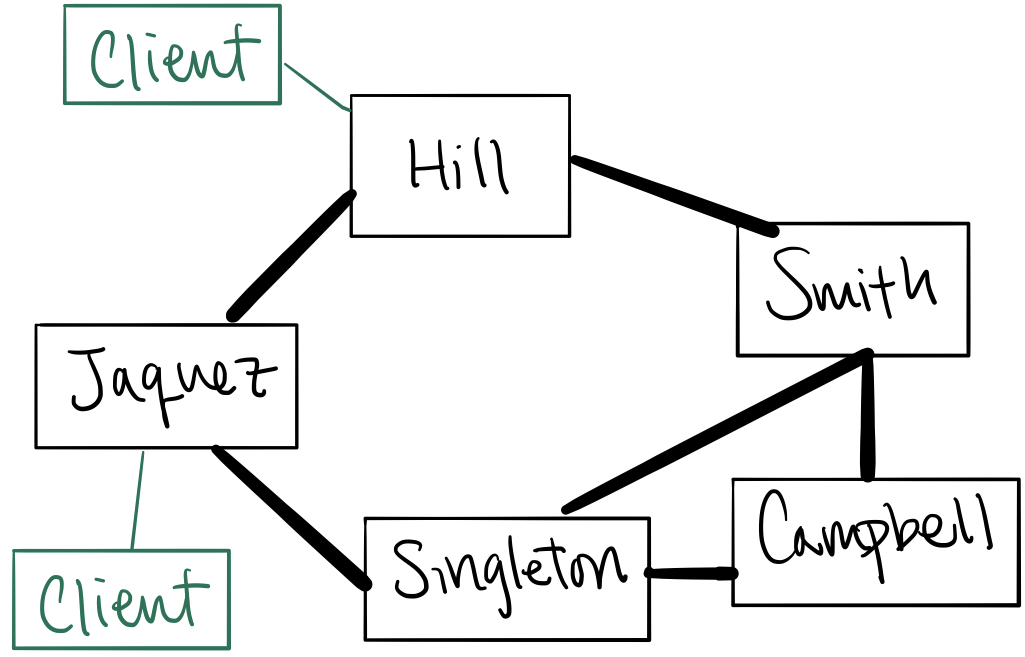
\includegraphics[scale=0.23]{server_connections.jpeg}
\caption{\label{fig:vectors} Diagram of Connections between Server Herds}
\end{figure}
%% %---------------------------
\subsection{WHATSAT Requests}
WHATSAT Requests are sent from client to server to ask what is near one of its clients. The requests are of the following form:
\begin{center}
    WHATSAT <Client ID> <Radius> <Max \# of Results>
\end{center}
The request is considered invalid if server does not contain any information about client specified in <Client ID>. WHATSAT request can be sent to any server in the herd even if that server was not the one who received the original IAMAT request from <Client ID>. The point is that all server should contain information about any client that has made request to any of the server in the herd. \par
No flooding is needed for WHATSAT Requests. Server that received the request calls the Google Places API via the aiohttp library, which on successful calls returns a JSON result of nearby locations. Server then formats the JSON result based on the client's specifications. The JSON library in Python was used to format received JSON object. Server returns the original IAMAT request made by <Client ID> and the result from Google Places API appended. 

\subsection{Server-to-Server Communication}
Server propagates location of client to neighboring servers once it receives a valid IAMAT Request or a valid propagated message from another server. With the asyncio library, servers can easily establish connection with other servers via a TCP connection similar to one established from client to server. The \texttt{open\_connection} method of asyncio will return a pair of (reader, writer) objects that server can use to communicate with designated server. Connection with designated server is closed once information is propagated. Note that only propagated message that have not been received by server is propagated.

\subsection{Difficulties Encountered}
Some of the difficulties I encountered during my implementation of the server herd prototype was how to deal with event loops in the Asyncio Library. The documentations of Asyncio online has many functions that are about how to start event loops and add tasks, but at the start I wasn't quite sure which function I should use. Nevertheless, I was able to figure out by looking through sample hint code provided by the TAs and writing simpler test code with functions related to event loops.

%-------------------------------------------------------------------------------
\section{Pros and Cons of Asyncio in Server Herd}
%-------------------------------------------------------------------------------
With Python and the Asyncio Library, we can easily write programs that run and exploit server herds as the concept of coroutines in Asyncio allows server to deal with multiple incoming requests and there are many built-in functions of the Asyncio Library that we can use and do not have implement from scratch. For example, the \texttt{start\_server} function allows us to start a socket server by simply passing in IP address, port, and a callable/corountine function that we want to the server to run. The callable/corountine function will then have access to reader and writer pair that can be easily used for client/server communication. In other frameworks and programming languages, many require much more complicated means to establish TCP connection between client and server. \par
In addition to built-in support for client/server connection, the Asyncio Library also contains built-in functions that supports cross-server TCP communication, such as \texttt{open\_connection} that also returns reader and writer pair to caller. With Asyncio's cross-server support, even implementing a server herd larger than 5 will not be a challenge. There are also external libraries that we can use together with the Asyncio Library to build more complicated servers, such as aiohttp that enables servers to send HTTP request to web APIs. \par
Nevertheless, the obvious downside of the Asyncio Library for implementing Server Herd is that it is single-threaded like most parts of Python, meaning it has limited parallelism capabilities and lacks support for multi-threaded programs. As mentioned before, the Global Interpreter Lock in Python allows only one thread who holds the global lock to execute at one time. Compared to other programming languages and frameworks that supports multi-threading, Python and Asyncio is at a disadvantage as multi-threading can help speed up intensive tasks that server may be requested to handle. \par
Another potential downside of the Asyncio Library is that it is a cooperative multitasking library where tasks voluntarily yield instead of being forcefully yielded by the scheduler. With this, there is the possibility of encountering a task that decides to not yield the global lock and continue to occupy the CPU, all other tasks that are waiting to be executed will never be executed. A preemptive multitasking approach can solve the problem, but it also comes with other downsides. \par
One other downside to consider is that with asynchronous functions in the Asyncio Library, it is very likely that our code will execute out of order and it is hard to determine the actual order of how our code will be executed due to different factors. With 5 servers, we do not see problems with our servers that arise from asynchronous executions. However, if we significantly increase the number of servers in our herd and the number of requests they receive, we may encounter case where an IAMAT Request arrive before a WHATSAT Request, but due to the asynchronous execution of different coroutines, there is a chance that the WHATSAT request will be processed prior to the IAMAT Request which would lead to an error. 
%-------------------------------------------------------------------------------
\section{Asyncio vs. Node.js}
Python and JavaScript are both dynamically typed languages with tricky behaviors at parallelism. They both support a single-threaded design which makes threads-based parallelism hard to implement. They both have libraries that provide asynchronization, Asyncio for Python and Node.js for JavaScript. They both have event loops as well. The asynchronous characteristic of the two frameworks are similar. Instead of coroutines in Python, Node.js uses the concept of callbacks, but both are part of the main event loop. Keywords such as \texttt{async} and \texttt{await} exists in both frameworks and have similar uses. Overall, they are similar in many ways, but it is important to note that asynchronization is not default solution of Node.js for concurrency problems. 
%-------------------------------------------------------------------------------
%-------------------------------------------------------------------------------
\section{Dependence on Asyncio Python 3.8 Features}
%-------------------------------------------------------------------------------
The function \texttt{asyncio.run()} graduated to stable API in Python 3.8. It can be used to execute a coroutine and return the result while automatically managing the event loop. It is noted in the Asyncio documentation that \texttt{asyncio.run()} should be the preferred way of running asyncio programs. The implementation of server herd prototype will be more concise using the \texttt{asyncio.run()} function, but it is not very difficult to get by with older version of Python as there are workarounds shown on documentation of Asyncio. We can manually create event loops using \texttt{asyncio.new\_event\_loop()}, execute loop with \texttt{asyncio.run\_until\_complete()}, and other built-in functions to model behavior of \texttt{asyncio.run()}. \par
Another feature that does not exist in previous Python versions is the command \texttt{python -m asyncio} which launches a natively async REPL(similar to a command prompt). This feature is useful when executing Python code in the style of commands, however, for our purpose, we mainly execute python files, so this feature is not heavily relied on. Thus, new features in Python 3.8 are very convenient, but they are not crucial as many workarounds exist for the new features.
%-------------------------------------------------------------------------------
\section{Conclusion}
%-------------------------------------------------------------------------------
In this project, we explored Python as a programming language and Asyncio as a framework for implementing an "application server herd" and evaluated its performance through research and implementation of a server herd prototype. Overall, Python and the Asyncio Library is suitable for implementing a server herd as major advantages include the concept of corountines and event loops in Asyncio, in addition to many built-in support for not only client/server communication, but also server/server communication. It lacks in certain areas in contrast to Java such as multi-threading capabilities and garbage collection for circular references, but these areas are less relevant to implementing the server herd of our desired scale. Thus, I would recommend using Python and the Asyncio Library to implement the new Wikimedia-style service.  
%-------------------------------------------------------------------------------
\section*{Acknowledgments}
%-------------------------------------------------------------------------------

Thank you to Professor Eggert and the TAs for introducing and grading our homeworks.

%-------------------------------------------------------------------------------

%-------------------------------------------------------------------------------

\newpage
\bibliographystyle{plain}
\bibliography{\jobname}
\\
Python 3.8 Asyncio Documentation \\
\url{https://docs.python.org/3/library/asyncio-stream.html#asyncio.open_connection} \\
Python 3.8 Event Loop Documentation \\
\url{https://docs.python.org/3/library/asyncio-eventloop.html} \\
TA Patricia Xiao and TA Kimmo Karkkainen's Slides \\
Memory Management in Python \\
\url{https://realpython.com/python-memory-management/} \\
Intro to Async Concurrency in Python vs. Node.js \\
\url{https://medium.com/@interfacer/intro-to-async-concurrency-in-python-and-node-js-69315b1e3e36}
Python Global Interpreter Lock \\
\url{https://wiki.python.org/moin/GlobalInterpreterLock} \\
Python 3.8 New Features \\
\url{https://docs.python.org/3/whatsnew/3.8.html#asyncio} \\
Garbage Collection in Java \\
\url{https://medium.com/computed-comparisons/garbage-collection-vs-automatic-reference-counting-a420bd4c7c81} \\

%%%%%%%%%%%%%%%%%%%%%%%%%%%%%%%%%%%%%%%%%%%%%%%%%%%%%%%%%%%%%%%%%%%%%%%%%%%%%%%%
\end{document}
%%%%%%%%%%%%%%%%%%%%%%%%%%%%%%%%%%%%%%%%%%%%%%%%%%%%%%%%%%%%%%%%%%%%%%%%%%%%%%%%

%%  LocalWords:  endnotes includegraphics fread ptr nobj noindent
%%  LocalWords:  pdflatex acks